\chapter{CODE VERIFICATION}
\label{chap:model_analysis}
The purpose of a numerical simulation is generally to accurately predict the behavior of a real system.
All mathematical modeling and numerical calculation, however, deals only with approximations.
It is therefore crucial to understand the degree to which these approximations reflect the actual scenario of interest, and to what extent their predictions can be trusted.
In this Chapter, the validity of the numerical approximations to the continuum model is discussed.
Concepts relating to determining the correctness of a whole code of specific results are surveyed.
The Fortran implementations of the finite difference and asymptotic solutions of the radiative transfer equation are verified to be free of detectable coding mistakes.

\section{Sources of Error in Numerical Simulations}
While simulations attempt to realistically reproduce real--life observations, many factors conspire to distort the numerical results they produce.
The following is an overview of the errors incurred throughout the process of creating and evaluating numerical models.
Some of these errors are \textit{ordered}, meaning that they can be decreased predictably by performing additional computations, while others are not.

First, any mathematical model is based on simplifying assumptions compared to the real system.
Any assumptions which do not hold precisely for the real system contribute to differences between model outputs and the real behavior.
Such differences can be termed \textit{conceptual modelling errors}, and are a present in the exact solutions to the mathematical equations comprising the model.
Once a model is formulated, it contains free parameters which can be varied to emulate different physical scenarios.
To evaluate the model, specific parameters must be used which reflect the scenario of interest.
The values of these parameters often are obtained experimentally, and may not be known with exact precision.
Error resulting from inaccurate physical parameter values can be called \textit{parameter uncertainty error}.

Mathematical models accurate enough to be useful are usually difficult or impossible to solve analytically.
Therefore, either mathematical simplifications or numerical approximations, or both, may be employed in order to obtain a solution.
For example, in the low--scattering solution presented in Section \ref{sec:symbolic_asymptotics}, the exact solution is expanded in a Taylor Series, from which only the first few terms are used, with the rest discarded.
The error resulting from using a finite number of terms from an infinite series is refered to as \textit{truncation error}.
Truncation error is ordered, as an arbitrary number of terms can be used to better approximate the true solution.
When a continuous equation is solved numerically, it is necessary to compute the solution on a finite number of discrete points rather than on the complete domain.
The error incurred by doing so is called \textit{discretization error}.
Discretization error is also ordered, as arbitrarily fine grids can be chosen in order to better approximate the continuum solution.

Finally, once the model, solution algorithm, and discretization scheme are chosen, a computer is used to perform the actual calculations.
Computers do not operate on the full set of real numbers, but rather on a finite subset of the real numbers with a predetermined floating point precision, depending on the hardware and software environment.
The loss of accuracy in computations due to the use of floating point numbers is termed \textit{round--off error}.


\section{Verification and Validation}
\label{sec:v2}
%TODO: Citations
As Roache explains, there are two aspects to building confidence in numerical codes, specifically those which solve PDEs:
verification deals with \textit{solving the equations right}, while validation deals with \textit{solving the right equations}.
Validation involves comparison with experimental evidence in order to determine that governing equations
accurately describe physical phenomenon, and that their solutions match observation.
That is, it is the process of checking that conceptual modelling errors are sufficiently small to model the system as accurately as necessary.
Validation is an ongoing process; as new experimental data become available, the equations can be solved under appropriate conditions in an attempt to replicate the new observations.
Verification, however, is a purely mathematical exercise, and has nothing to do with the physical system being modeled.
It deals only with the agreement between an equation and its numerical solution produced by a particular implementation of an algorithm.
It involves checking that ordered sources of numerical error (truncation and discretization errors) decrease as expected when additional computations are performed.
Unlike validation, verification is something to be started and finished.
If a set of parameters to the model can be chosen to exercise all terms in the equation, comparison between the numerical and exact solution is sufficient to demonstrate the correctness of a computational code, and the process need not be repeated unless the code is modified.

Due to lack of sufficient experimental data, rigorous validation of the present radiative transfer code is left as future work.
However, verification of both the finite difference and numerical asymptotics algorithms is demonstrated here.
There are two phases of verification.
The first is \textit{code verification}, where the overall implementation of an algorithm is tested, and the difference between the numerical and analytical solutions is \textit{explicitly measured} at every point in the numerical solution.
The same calculation is repeated for several grid sizes, and it is checked that the convergence order as the grid spacing approaches zero matches the theoretical convergence order of the algorithm.
The explicit measurement of errors requires that the analytical solution be known, which is generally only possible for some unrealistic or uninteresting set of parameters.
If the analytical solution were available for the real, interesting case, then it would probably not have been necessary to implement a numerical solution in the first place.
Nevertheless, analyzing a well--chosen unrealistic situation is sufficient to check that the order of the code's discretization error matches the theoretical order of the algorithm.

For realistic conditions, however, a second stage of verification is emplyed: \textit{verification of calculations}.
In this phase, a specific calculation of interest is performed, and the error is \textit{estimated} since it cannot be measured explicitly when the exact solution is not available.
This is generally done by repeating the calculation for several grid sizes, as above, then using a technique called Richardson Extrapolation to estimate the limiting solution as the grid spacing approaches zero.
This estimated limiting solution is then compared to the actual numerical solutions.
Since the solutions are known on different grids, they cannot be compared pointwise without interpolation.
Rather, a single scalar calculated from some integral of the solution is often used as a simple measure of the global order of accuracy. %TODO: CITE 2008_Procedure

\section{Code Verification: Method of Manufactured Solutions}

The most obvious way to obtain an analytical solution to compare to a numerical solution is by choosing a simple case where the PDE can be solved explicitly, perhaps through separation of variables or by reducing it to an ODE.
This is referred to as the method of exact solutions (MES).
However, such simple cases usually result in such a loss of generality that they become useless in testing the complicated aspects of the solution algorithm.
In order to verify that a code will work in an interesting case, every term in the equation must be exercised during the verification process.
An alternative process, the method of manufactured solutions (MMS), retains arbitrary generality in the equations while making analytical solutions readily available.
Of course, there is a trade-off: the solutions are not physically realistic.
However, this is not an issue; as stated previously, \textit{verification is a purely mathematical endeavor}.
Determining that a code solves an equation correctly is unrelated to physical realism.

The method of manufactured solutions is performed as follows.
Consider a differential equation
\begin{align}
  Du(\vec{x}) = \sigma(\vec{x}), \label{eqn:mms_de} \\
  u(\vec{x})=f(\vec{x}) \mbox{ for } \vec{x} \in \Sigma,
  \label{eqn:mms_bc}
\end{align}
where $D$ is a differential operator, $u$ is the solution, $\sigma$ is a source term, $f$ is the boundary condition function, and $\Sigma$ is the set of boundary points at which the boundary condition is applied.
Normally, $D$, $\sigma$, and $f$ are known, and solving for $u$ involves determining $D^{-1}$ and calculating $u = D^{-1}\sigma$ subject to \eqref{eqn:mms_bc}.

The Method of Manufactured Solutions reverses the normal procedure.
Here, $u$ is hand-picked at the outset to be easy to calculate, all parameters and coefficient functions in $D$ are chosen to be nonzero, and the source term $\sigma$ which produces the desired solution is calculated.
Similarly, the boundary condition is determined from the chosen solution.
In essence, rather than solving $u = D^{-1}\sigma$ subject to $u(\Sigma)=f$, it suffices to compute $\sigma = Du$ and evaluate $f=u$ at the boundary.
Whereas \textit{inverting} a differential operator analytically is impossible for many equations and often requires ingenuity when it is, \textit{applying} one is a plug-and-chug application of algebra and calculus.
Of course, it is necessary to construct $u$ and any coefficient functions in $D$ from simple, differentiable and integrable functions.

Also, $u$ must satisfy any constraints imposed by the algorithm such as hard-coded boundary conditions or acceptable coefficient ranges.
Finally, the chosen functions should have small derivatives so that convergence can be achieved for reasonable grid sizes.
Since these functions may need to be fairly complicated in order to achieve full generality while meeting the necessary constraints, it is advisable to use a \textit{Computer Algebra System} (CAS) such as the Python package Sympy to symbolically compute the source term. % TODO: Cite Sympy

\subsection{Discretization Error Analysis}
Once an exact solution is known, code verification is performed by demonstrating that the discretization error of the code matches the theoretical order of accuracy of the algorithm.
Numerical calculations are computed on a sequence of discrete grids from coarse to fine, and errors are calculated by evaluating the exact soution pointwise.
Then, some norm (usually $l_1$, $l_2$, or $l_\infty$) of the discretization error is calculated for each grid.
To verify an algorithm of order $p$ with grid resolution $h$, it should be shown that the norm of the pointwise error is approximately proportional to $h^p$.

This effect occurs only for small grid resolutions, when the first nonzero term in the error series dominates the others.
If large grid spacings are used, then order $p$ convergence may not be observed even in a correct implementation since higher order error terms will overpower the order $p$ term.
The range of small grid spacings for which the lowest order term dominates is known as the \textit{asymptotic range} (a.k.a. ``the sweet spot'').
If the verification procedure shows that the implementation does not demonstrate the theoretical order of accuracy of the algorithm, this is most likely an indication that either a coding mistake is present or the asymptotic range has not been achieved. % TODO: Cite roache after "most likely"

\subsection{Synthetic Data}
\label{sec:synthetic_data}
In order to perform code verification for the radiative transfer equation, it is necessary to first choose a manufactured solution $L(\vec{x}, \vec{\omega})$ for radiance, as well as coefficient functions for the absorption coefficient $a(\vec{x})$ and volume scattering function $\beta(\vec{\omega}\cdot\vec{\omega'})$.
Together, the chosen solution and coefficient functions are referred to as \textit{synthetic data}.
The code developed for this thesis imposes the following conditions on the manufactured solution:
\begin{enumerate}
  \item Periodic solution and absorption coefficient in $x$ and $y$
  \item Positive solution and absorption coefficient
  \item Position-independent surface downwelling boundary condition
  \item Zero upwelling radiance at the bottom boundary
  \item Properly normalized VSF $\beta(\Delta)$, as described in Section \ref{sec:iops}
\end{enumerate}
The actual expressions chosen for the synthetic data are quite unwieldy, and are listed in full in Appendix \ref{chap:synthetic_data}.


% TODO: Revise
\subsection{Finite Difference Verification}
% TODO: Discuss OAMs (order of accuracy mistakes)
%The only source of error in the finite difference method is discretization error due to the truncation of terms in the Taylor Series during the construction of the finite difference formulas in Section \ref{sec:discretization}.
Since second order finite difference formulas are used, once the asymptotic range for grid spacing has been achieved, decreasing it further should result in the discretization error approaching zero quadratically.
The radiative transfer equation involves five discretized variables: $(x,y,x,\theta,\phi)$.
A five dimensional resolution space is nontrivial to characterize, so we define generic spatial and angular resolutions for the sake of reducing dimensionality,
Let $n_s = n_x = n_y = n_z$ and $n_a = n_\theta = n_\phi$.
Then, we use the geometric mean to describe the spatial and angular resolution, as
\begin{align}
  ds &= (dx\, dy\, dz)^{1/3}, \\
  da &= (d\theta\, d\phi)^{1/2}.
\end{align}

This reduces the dimenionality of the resolution space to two, but it would be preferrable to deal only with a single variable.
Therefore, the finite difference verification is performed by holding $n_a=8$, and varying $n_s$ between 4 and 64.
As shown in Figure \ref{fig:fd_mms}, second order convergence is observed, demonstrating that the code works without order-of-accuracy mistakes.
% TODO: Discuss multidimensional error further
% TODO: Discuss log-log plot.

\begin{figure}[h]
  \centering
  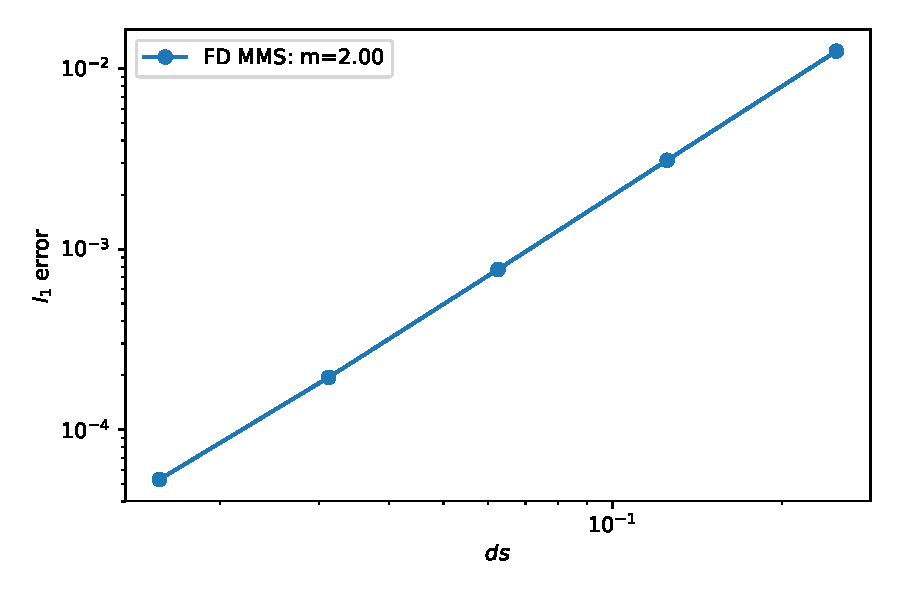
\includegraphics[width=5in]{fd_mms}
  \caption{Code verification for the finite difference solution. Each point represents the same simulation run with a different spatial grid sizes, with the angular grid held constant at $n_a=8$. A slope of $m=2$ on a log-log scale demonstrates second order convergence, as expected, demonstrating the correctness of the code.}
  \label{fig:fd_mms}
\end{figure}

\subsection{Numerical Asymptotics Verification}
\label{sec:num_asym_mms}
For the numerical asymptotics algorithm, both discretization error and truncation error are present.
Therefore, the solutions are not expected to converge to the true solution by increasing the grid size.
Neither is it guaranteed that increasing the number of terms will lead to convergence to the true solution.
However, while the discretization error is not verifiable in that sense, the truncation error \textit{is}.
That is, since the $n$--term asymptotic solution is a numerical approximation to the $n$--term Taylor series, the norm of the pointwise error should decrease with order $n+1$ as $b \to 0$.
As with discretization error, this can only be observed within some asymptotic range of small $b$ values higher order error terms dominate for large values of $b$.

Figure \ref{fig:mms_asym_b_conv} demonstrates the convergence of the asymptotic solution as $b \to 0$.
The first three approximations are reasonably close, to demonstrating order $n+1$ convergence, but the $n=3$ approximation converges slower than expected.
It is unclear whether this is due to a coding mistake, the effect of discretization error, or if there is another cause for the sub-optimal convergence.
\begin{figure}[h]
  \centering
  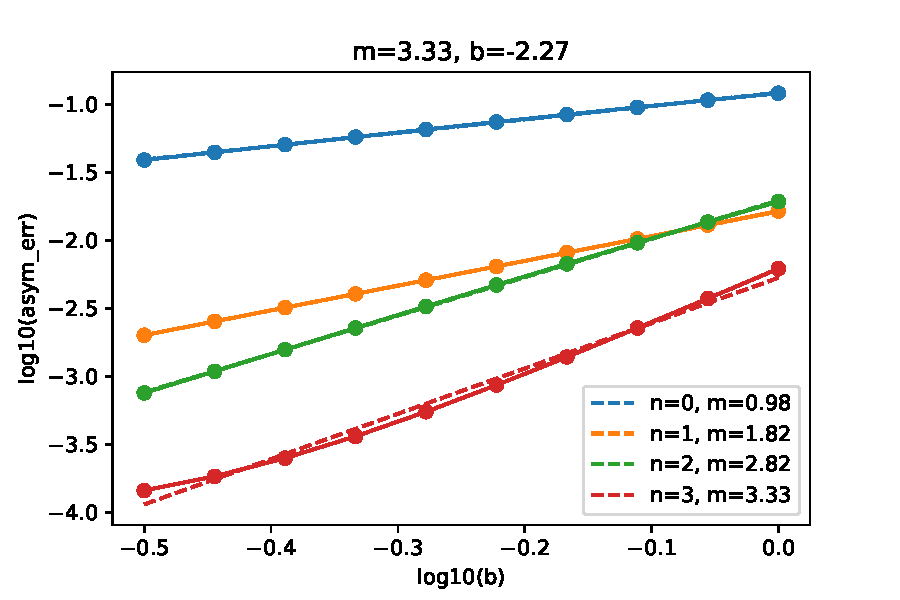
\includegraphics[width=5in]{mms_asym_b_conv}
  \caption{Code verification for the numerical asymptotics solution via the Method of Manufactured Solutions. A range of $b$ values are run, using 0 - 3 terms in the asymptotic series. The legend shows the number of terms ($n$) and the observed convergence order ($m$) for each solution.}
  \label{fig:mms_asym_b_conv}
\end{figure}

\section{Verification of Calculations}
As mentioned in Section \ref{sec:v2}, numerical error can be estimated for realistic simulations for cases when the exact solution is not known by analyzing the convergence of a scalar functional of the numerical solution over several grid sizes.

\subsection{Richardson Extrapolation}
Richardson extrapolation is a technique for estimating the continuum value of a scalar functional derived from a solution to a differential equation by using values of the scalar obtained from numerical solutions on several different grids.
The technique was developed by Richardson in 1912 with an application paper related to a stresses on a dam, and is also known as $h^2$ extrapolation since it was originally applied to a second order method.
The basic concept is as follows.

Let the scalar of interest be called $\phi$ and the grid spacing $h$.
Denote the exact solution as
\begin{equation}
  \phi_e = \lim_{h \to 0} \phi(h),
\end{equation}
The crux of the technique is to assume that discretization error can be written as a linear combination of powers of $h$, as in a Taylor series.
That is,
\begin{equation}
  \phi - \phi_e = g_0 + g_1 h + g_2 h^2 + g_3 h^3 + \cdots.
\end{equation}
Assuming that a second order numerical method is used, the first two terms on the right hand side are zero.
For a first order method, only the first term is necessarily zero.
Of course, in a ``zeroth order'' method, the absolute error is bounded from below by $|g_0|$, and so does not approach zero as the grid is refined.
``Zeroth order'' methods are also known as ``incorrect.''

The original technique involves numerical solutions on two grids with spacings $h_1 < h_2$ (i.e., grid 1 is finer), from which scalars $\phi_1$ and $\phi_2$ are calculated.
The ratio $r = h_2/h_1$ is called the grid refinement ratio.
Then,
\begin{align*}
  \phi_1 &= \phi_e + g_2 h_1^2 + O(h^3), \\
  \phi_2 &= \phi_e + g_2 h_2^2 + O(h^3).
\end{align*}
Solving for $g_2$ yields
\begin{equation*}
  g_2 = \frac{\phi_1 - \phi_e}{h_1^2} + O(h^3), \\
\end{equation*}
so
\begin{align*}
  \phi_1 &= \phi_e + \frac{h_2^2}{h_1^2}(\phi_1 - \phi_e) + O(h^3) \\
  &=  \phi_e + r^2(\phi_1 - \phi_e) + O(h^3) \\
  &= \phi_e(1-r^2) + \phi_1 r^2 + O(h^3).
\end{align*}
Hence, the approximate continuum solution is
\begin{equation*}
  \phi_e = \frac{\phi_2 - \phi_1 r^2}{1 - r^2} + O(h^3).
\end{equation*}
In essence, Richardson extrapolation allows for $\phi$ values from two solutions from an order $h^p$ numerical method to be combined to produce an approximation of order $h^{p+1}$ to the continuum value of $\phi$.

\subsection{Generalized Richardson Extrapolation}
Of course, the above equations are only approximations.
In reality, higher order terms introduce noise which may distort the extrapolated value
when only two grid sizes are used.
In order to reduce this noise, the concept can be easily generalized to incorporate more than two numerical solutions, as follows.
From
\begin{equation*}
  \phi \approx \phi_e + g_2 h^2,
\end{equation*}
it is clear that $\phi$ is approximately linear in $h^2$.
Therefore, a simple linear fit through multiple points in $(h^2, \phi)$ space yields $\phi_e$ as the $\phi$--intercept.
The slope, $g_2$, can be discarded.
If significant noise due to outliers still distorts the extrapolated values during fitting, a robust fitting algorithm such as Huber \cite{yu_robust_2014} or Ridge \cite{hoerl_ridge_1970} regression can help reduce the influence of outliers.

Additionally, this take on Richardson extrapolation is trivially applied to multiple dimenisions.
For a grid which has several resolution parameters $h_1, h_2, \ldots, h_n$ (e.g. multiple spatial dimensions, or spatial and angular grid resolutions), if the algorithm is second-order in each resolution parameter, then
\begin{equation*}
  \phi \approx \phi_e + g_{21} h_1^2 + g_{22} h_2^2 + \ldots + g_{2n} h_n^2.
\end{equation*}
Hence, fitting a plane or hyper-plane through several points in $(h_1^2, h_2^2, \ldots, h_n^2, \phi)$ space similarly produces $\phi_e$ as the $\phi$--intercept.
